\documentclass[11pt, headheight=30pt]{scrartcl}
\usepackage[hw]{darkWhite}

\newcolumntype{L}{>{$}l<{$}} % math-mode version of "l" column type
\newcolumntype{C}{>{$}c<{$}} % math-mode version of "c" column type

\DeclareMathOperator{\Mat}{Mat}
\DeclareMathOperator{\diag}{diag}


\title{18.755 Lie Algebra}
\subtitle{Homework 3}
\author{Rowechen Zhong with Isaac Zhu}
\begin{document}

% Proposition 30.11. (Skew Howe duality) Let V, W be complex vector spaces. Show that
% ∧
% n
% (V ⊗ W) ∼=
% M
% λ:|λ|=n
% S
% λV ⊗ S
% λ
% †W
% as GL(V ) × GL(W)-modules.

% Exercise 30.12. Prove Proposition 30.11.
% Hint: Repeat the proof of the usual Howe duality (Subsection 29.2),
% using Corollary 30.10.

\section{Skew Howe Duality}

\begin{prob*}
  Let $V, W$ be complex vector spaces. Show that
  \[
    \wedge^n (V \otimes W) \cong \bigoplus_{|\lambda| = n} S^\lambda V \otimes S^{\lambda \dagger} W
  \]
  as $GL(V) \times GL(W)$-modules.
\end{prob*}

\idea{
    [Hint]
    Repeat the proof of the usual Howe duality (Subsection 29.2), using Corollary 30.10.
}
$\wedge^n (V \otimes W)$ is naturally identified with the subspace of $(V \otimes W)^{\otimes n}$ which is antisymmetric under the action of $S_n$. Equivalently, this is the subspace of $V^{\otimes n} \otimes W^{\otimes n} \tensor \CC_{sgn}$ which is \emph{invariant} under $S_n$. Thus, by Schur-Weyl duality, we can expand as $GL(V) \times GL(W) \times S_n$-modules:
\begin{align*}
    V^{\tensor n} \tensor W^{\tensor n} \tensor \CC_{sgn} &\cong \left(
        \bigoplus_{|\lambda|=n} S^\lambda V \tensor \pi_\lambda
    \right)
    \tensor 
    \left(
        \bigoplus_{|\mu|=n} S^\mu W \tensor \pi_\mu
    \right) \tensor \CC_{sgn} \\
    &= \bigoplus_{|\lambda| = |\mu| = n} S^\lambda V \tensor S^\mu W \tensor \pi_\lambda \tensor \pi_\mu \tensor \CC_{sgn} \\
    &= \bigoplus_{|\lambda| = |\mu| = n} S^\lambda V \tensor S^\mu W \tensor \pi_\lambda \tensor \pi_{\mu^\dagger}\\
    &= \bigoplus_{|\lambda| = |\mu| = n} S^\lambda V \tensor S^\mu W \tensor \CC^{\delta_{\lambda, \mu^\dagger}}\\
    &= \bigoplus_{|\lambda| = n} S^\lambda V \tensor S^{\lambda^\dagger} W
\end{align*}
as desired.


% Exercise 30.13. Compute characters and dimensions of irreducible
% representations La+b,b,0 of SL3(C), where a, b ≥ 0. Compute the weight
% multiplicities and draw the weights on the hexagonal lattice for
% a + b ≤ 3, indicating the multiplicities. What are the special features
% of the case b = 0?
% Hint. The best way to do this exercise is to compute the characters
% recursively, using that V ⊗La+b,b,0 = La+b+1,b,0⊕La+b,b+1,0⊕La+b−1,b−1,0
% (if a = 0, the second summand drops out and if b = 0 then the third
% one drops out), by the “addable boxes” rule. This allows one to express
% the characters for b + 1 in terms of the characters for b and b − 1. And
% we know the characters of La,0,0 - they are the complete symmetric
% functions ha.

\section{Characters and Dimensions of Irreducible Representations}

\begin{prob*}
  Compute characters and dimensions of irreducible representations $L_{a+b,b,0}$ of $SL_3(\CC)$, where $a, b \geq 0$. Compute the weight multiplicities and draw the weights on the hexagonal lattice for $a + b \leq 3$, indicating the multiplicities. What are the special features of the case $b = 0$?
\end{prob*}

\idea{
    The best way to do this exercise is to compute the characters recursively, using that
    \[
        V \otimes L_{a+b,b,0} = L_{a+b+1,b,0} \oplus L_{a+b,b+1,0} \oplus L_{a+b-1,b-1,0}
    \]
    (if $a = 0$, the second summand drops out and if $b = 0$ then the third one drops out), by the ``addable boxes'' rule. This allows one to express the characters for $b + 1$ in terms of the characters for $b$ and $b - 1$. And we know the characters of $L_{a,0,0}$ - they are the complete symmetric functions $h_a$.
}

Instead of applying the hint, we're just going to use Weyl Character formula.
\[
    s_\lambda(x_1, x_2, x_3) = \frac{\det(x_i^{\lambda_j + N - j})}{\prod_{i < j}(x_i - x_j)}
\]
We can write out the full expression. The numerator is
\[
    \det\begin{pmatrix}
        x_1^{\lambda_1 + 2} & x_2^{\lambda_1 + 2} & x_3^{\lambda_1 + 2} \\
        x_1^{\lambda_2 + 1} & x_2^{\lambda_2 + 1} & x_3^{\lambda_2 + 1} \\
        x_1^{\lambda_3} & x_2^{\lambda_3} & x_3^{\lambda_3}
    \end{pmatrix}
\]
Plugging in $\lambda = (a+b, b, 0)$, we get
\[
    s_{a+b,b,0}(x_1, x_2, x_3) = \frac{\det\begin{pmatrix}
        x_1^{a+b+2} & x_2^{a+b+2} & x_3^{a+b+2} \\
        x_1^{b+1} & x_2^{b+1} & x_3^{b+1} \\
        1 & 1 & 1
    \end{pmatrix}}{(x_1 - x_2)(x_1 - x_3)(x_2 - x_3)}
\]

We could simplify this easily, but this is just more tedious calculations. Moving right along, the Weyl Dimension Formula is
\[
    \dim L_\lambda = \frac{\prod_{i < j}(\lambda_i - \lambda_j + j - i)}{\prod_{i < j}(j - i)}    
\]
In our case, we have
\[
    \dim L_{a+b,b,0} = \frac{(1+a)(1+b)(2+a+b)}{1 \cdot 2 \cdot 1} = \frac{(1+a)(1+b)(2+a+b)}{2}
\]

\begin{center}
    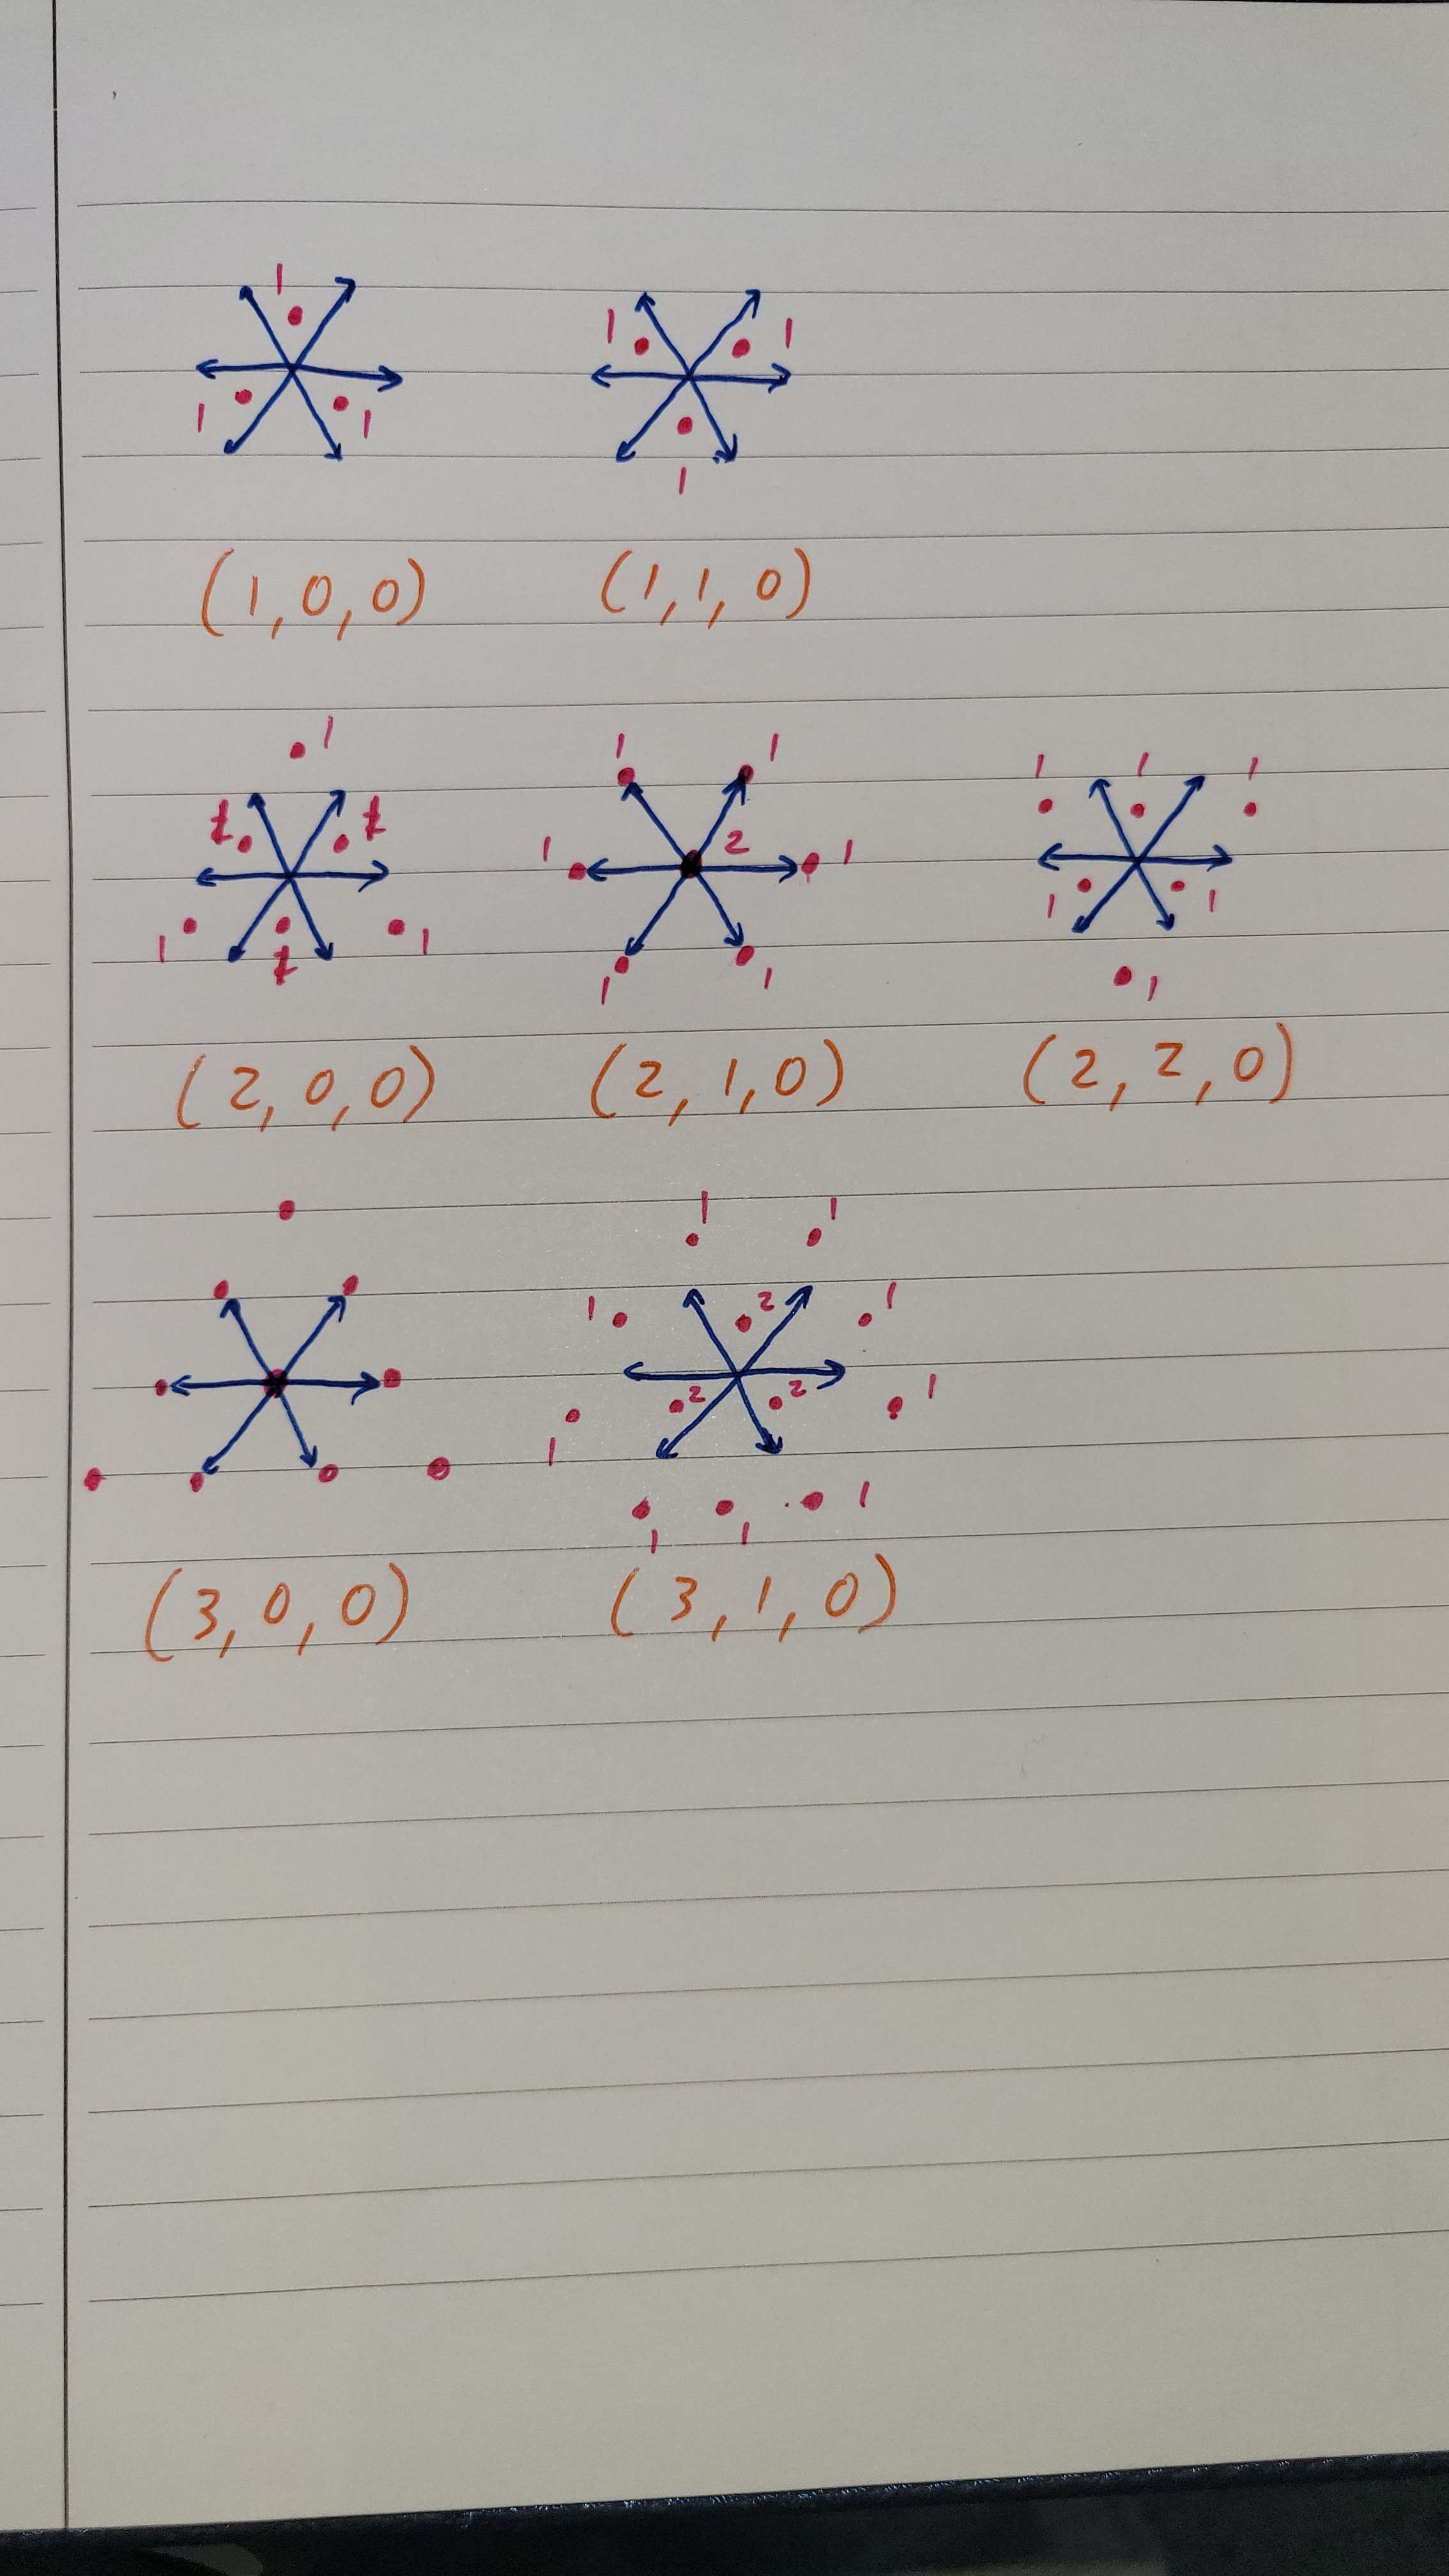
\includegraphics[width=0.5\textwidth]{hw3_hexagon.jpg}
\end{center}

I did not draw the $1$-dimension representation (a single point at the origin with dimension $1$) or $L_{3,2,0}$ (which is $L_{3,1,0}$ but flipped) and $L_{3,3,0}$ (which is $L_{3,0,0}$ but flipped).

% Exercise 30.14. Compute the decomposition of ∧
% mV ⊗ S
% kV ,
% ∧
% mV ⊗ ∧kV , S
% 2
% (∧
% mV ), ∧
% 2
% (∧
% mV ) into irreducible representations of
% GL(V ).

\section{Decomposition of Tensor Products}

\begin{prob*}
  Compute the decomposition of
  \[
    \wedge^m V \otimes S^k V, \quad \wedge^m V \otimes \wedge^k V, \quad S^2(\wedge^m V), \quad \wedge^2(\wedge^m V)
  \]
  into irreducible representations of $GL(V)$.
\end{prob*}

We know that $\wedge^m V \otimes L_\lambda = \bigoplus_{\mu \in \lambda + m} L_\mu$, where we sum over partitions obtained by adding $m$ addable boxes to different rows. We can use this to compute the decomposition of $\wedge^m V \otimes S^k V$ and $\wedge^m V \otimes \wedge^k V$:
\[
    \wedge^m V \otimes S^k V = \bigoplus_{\mu \in (k, 0, \ldots, 0) + m} L_\mu = L_{(k+1)(1^{m-1})} \oplus L_{(k)(1^m)}
\]
and
\[
    \wedge^m V \otimes \wedge^k V = \bigoplus_{\mu \in (1^k) + m} L_\mu = \sum_{i = 0}^{\min(m,k)} L_{(2^{i})(1^{m+k-2i})}
\]

The other two are a bit more difficult. Let me explicitly construct the highest weight vectors inside of $\wedge^m V \otimes \wedge^m V$. (We assume that the dimension of $V$ is sufficiently large; else some things simply vanish).
\[
    \sum_{T\subset \{\ell + 1,\dots, 2m - \ell\}, \abs{T} = m - \ell} \sgn(T) e_1\wedge\dots \wedge e_\ell \wedge e_{T_1} \wedge \cdots \wedge e_{T_{m-\ell}} \otimes e_1\wedge\dots \wedge e_\ell \wedge e_{\bar{T}_{1}} \wedge \cdots \wedge e_{\bar{T}_{m - \ell}}
\]
(here, $T$ is a subset of $\{\ell + 1,\dots, 2m - \ell\}$ of size $m - \ell$, and $\bar{T}$ is its complement; these are sorted, and $\sgn(T)$ is the parity of the sum of the elements in $T$).

This guy is obviously the highest weight of the representation $L_{(2^{\ell})(1^{2m - 2\ell})}$. Indeed, consider acting on this object to raise $\alpha+1$ to $\alpha$. If $\alpha \leq \ell$, this immediately vanishes. Else, if $\alpha$ and $\alpha + 1$ are both in $T$, or both in $\bar{T}$, the term vanishes. Else, suppose $T = (\dots, \alpha, \dots)$ and $\bar{T} = (\dots, \alpha + 1,\dots)$. This term in the sum pairs with $T = (\dots, \alpha + 1,\dots)$ and $\bar{T} = (\dots, \alpha, \dots)$, where we swap only $\alpha$ and $\alpha + 1$. This flips the sign, and both elements are raised to the same value, thus the whole sum vanishes.

These are all of them, because
\[
    (\wedge^m V)^{\otimes 2} = \bigoplus_{\ell\leq m } L_{(2^{\ell})(1^{2m - 2\ell})}
\]

In addition, it is symmetric if and only if $m - \ell$ is even. We conclude that
\[
    S^2(\wedge^m V) = \bigoplus_{\ell\leq m, m - \ell \text{ even}} L_{(2^{\ell})(1^{2m - 2\ell})}
\]
and
\[
    \wedge^2(\wedge^m V) = \bigoplus_{\ell\leq m, m - \ell \text{ odd}} L_{(2^{\ell})(1^{2m - 2\ell})}
\]

\end{document}